\documentclass{article}
\usepackage{graphicx}
\usepackage{amsmath}
\usepackage{listings}
\usepackage{geometry}
\geometry{margin=1in}

\title{Programming Assignment 2: Chaotic Dynamics of an Elastic Pendulum}
\author{Dimitri Bolt}
\date{}

\begin{document}
	
	\maketitle
	
	\section*{I. Sensitive Dependence on Initial Conditions}
	
	\begin{enumerate}
		\item Using the provided script \texttt{equations\_of\_motion.py}, we consider two slightly different initial conditions:
		\[
		\text{Initial Conditions} = \begin{bmatrix}
			1 & 1+10^{-4} \\
			\pi/6 & \pi/6 \\
			0 & 0 \\
			0 & 0
		\end{bmatrix}.
		\]
		The numerical integration clearly shows diverging trajectories over time, indicating strong sensitivity to initial conditions.
			\begin{figure}[h!]
				\centering
				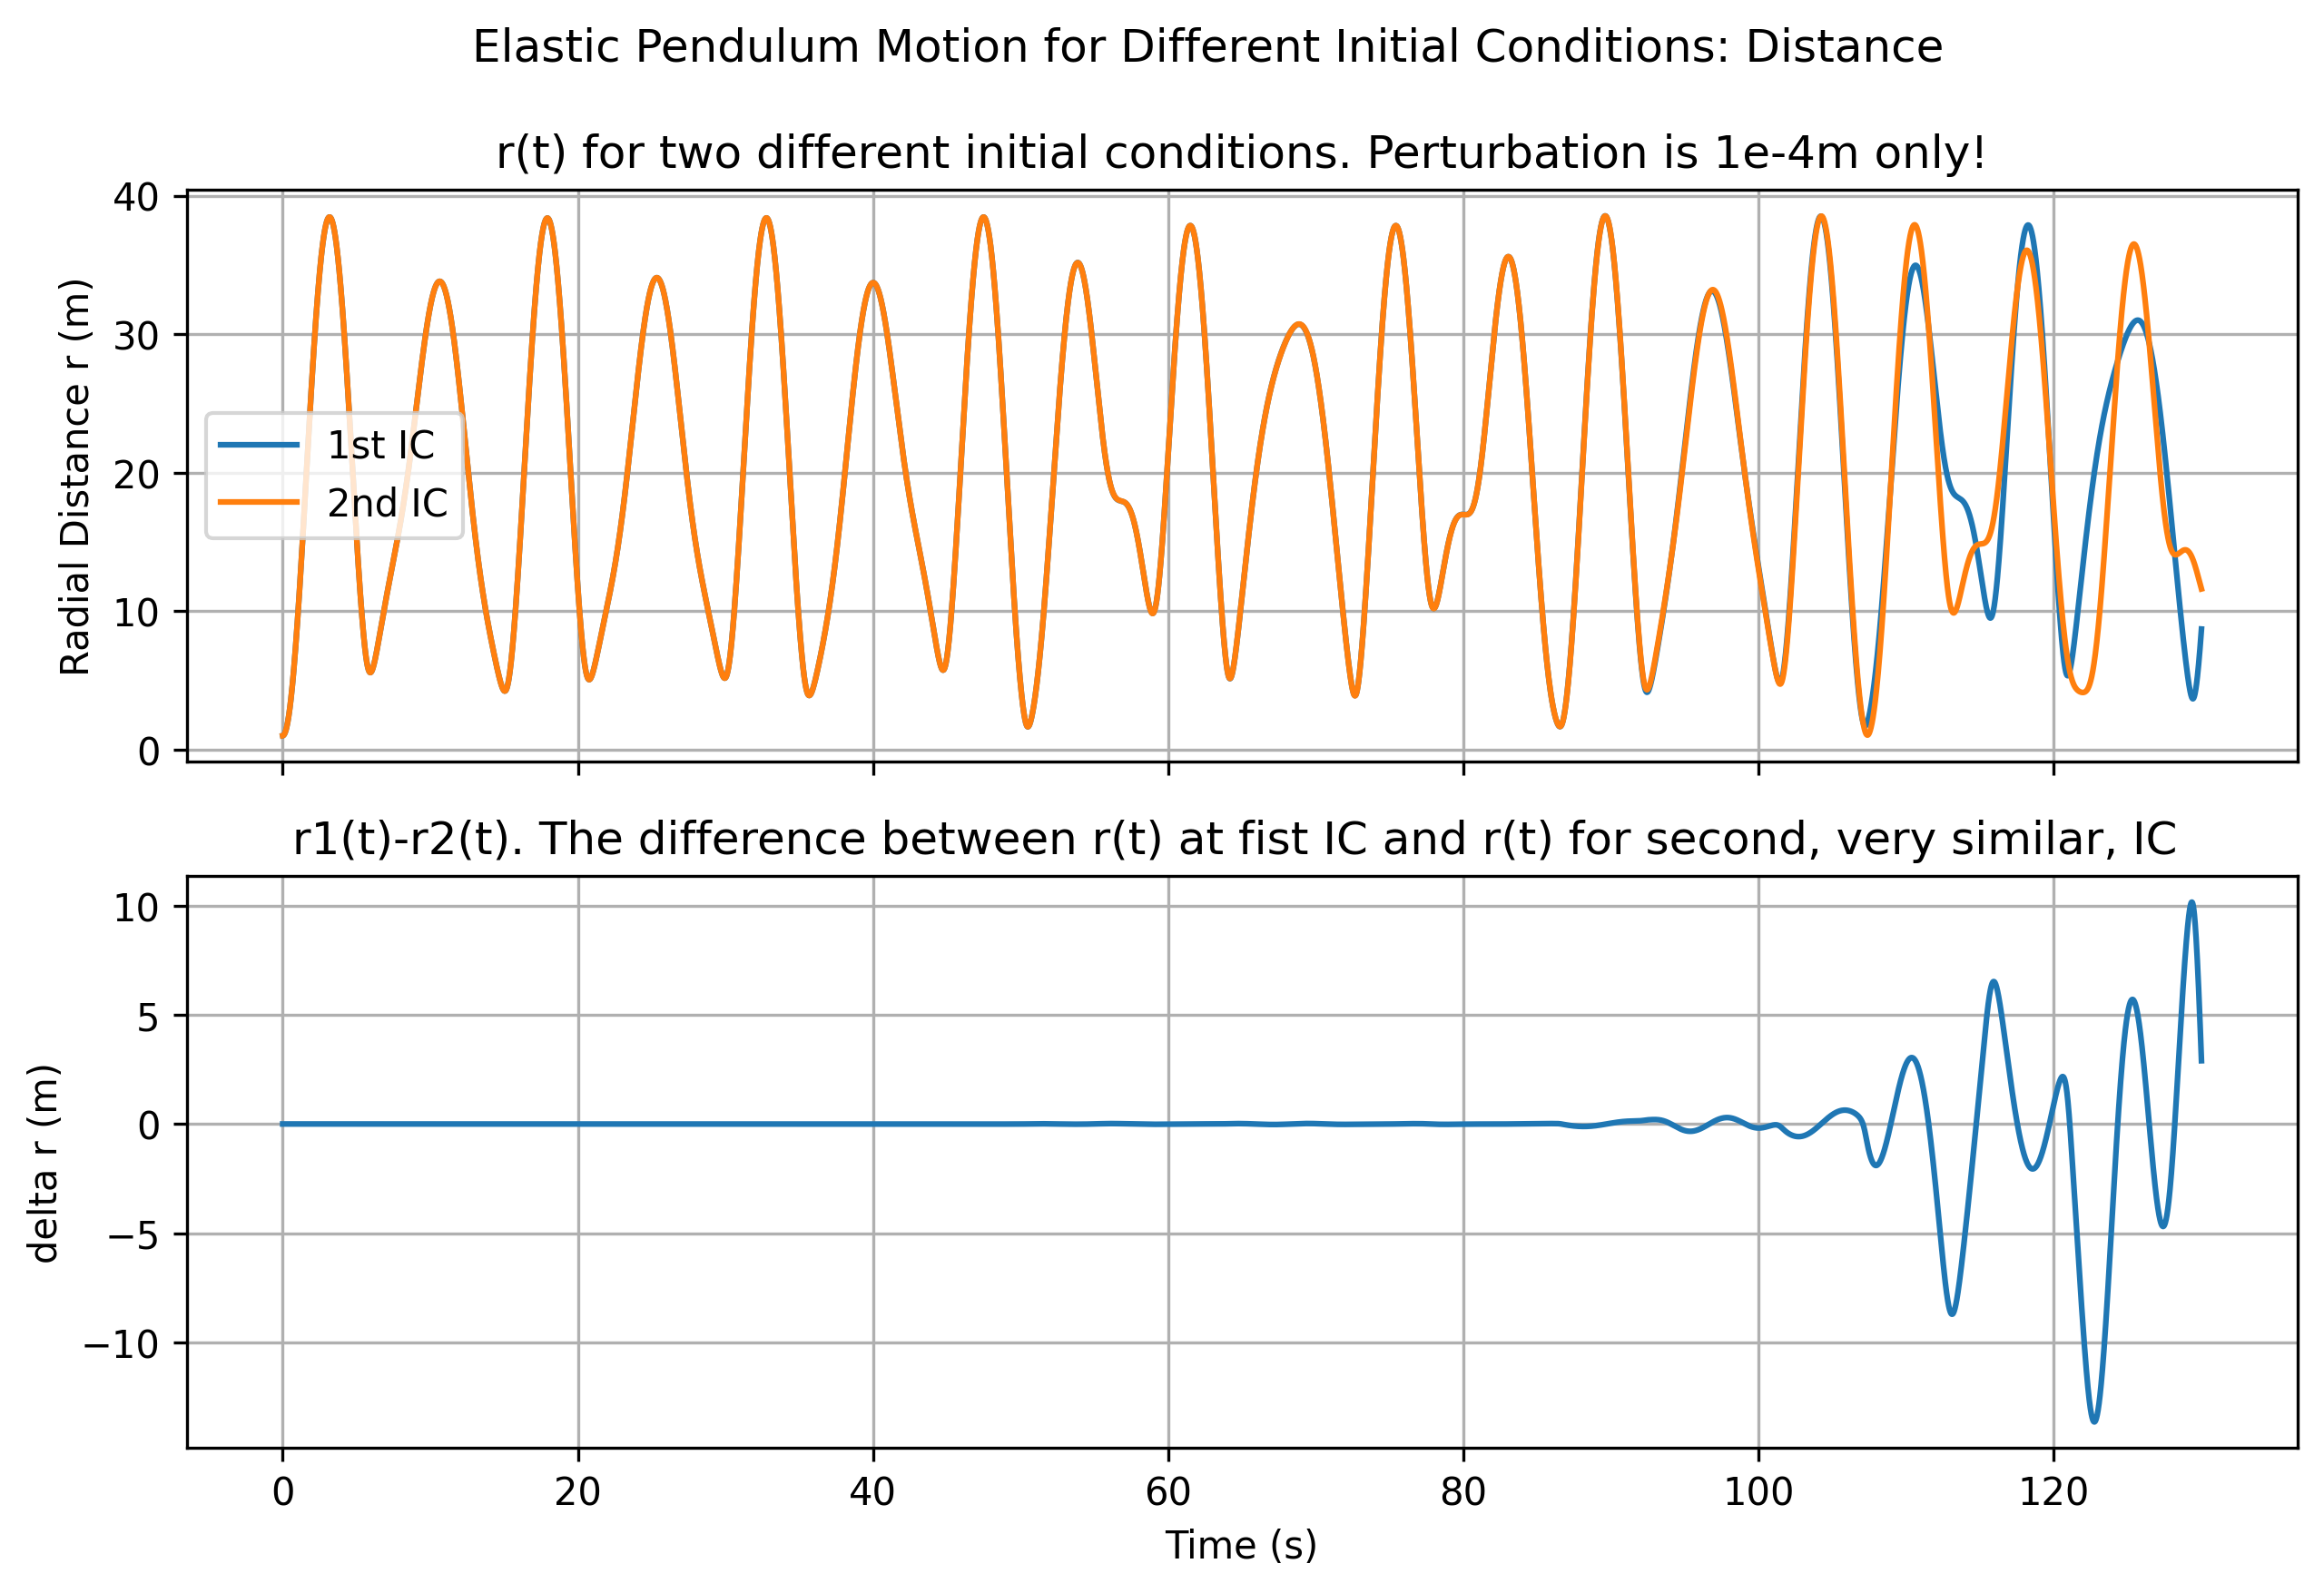
\includegraphics[width=0.8\textwidth]{elastic_pendulum_r.png}
				\caption{Distance and difference over time. Perturbation is 1e-4m only!}
			\end{figure}
		
		\item The difference in functions $r(t)$ can be observed clearly from the first and second charts on \texttt{Figure 1}. The differences are computed for the first initial condition and for the second.
		
		\item Differences in functions $\theta(t)$ are shown ion \texttt{Figure 2}.
		
		\item Even minute differences in initial conditions ($10^{-4}$ m) lead to significant divergence in trajectories due to the system's inherent nonlinearity and sensitive dependence, typical of chaotic systems.
			\begin{figure}[h!]
				\centering
				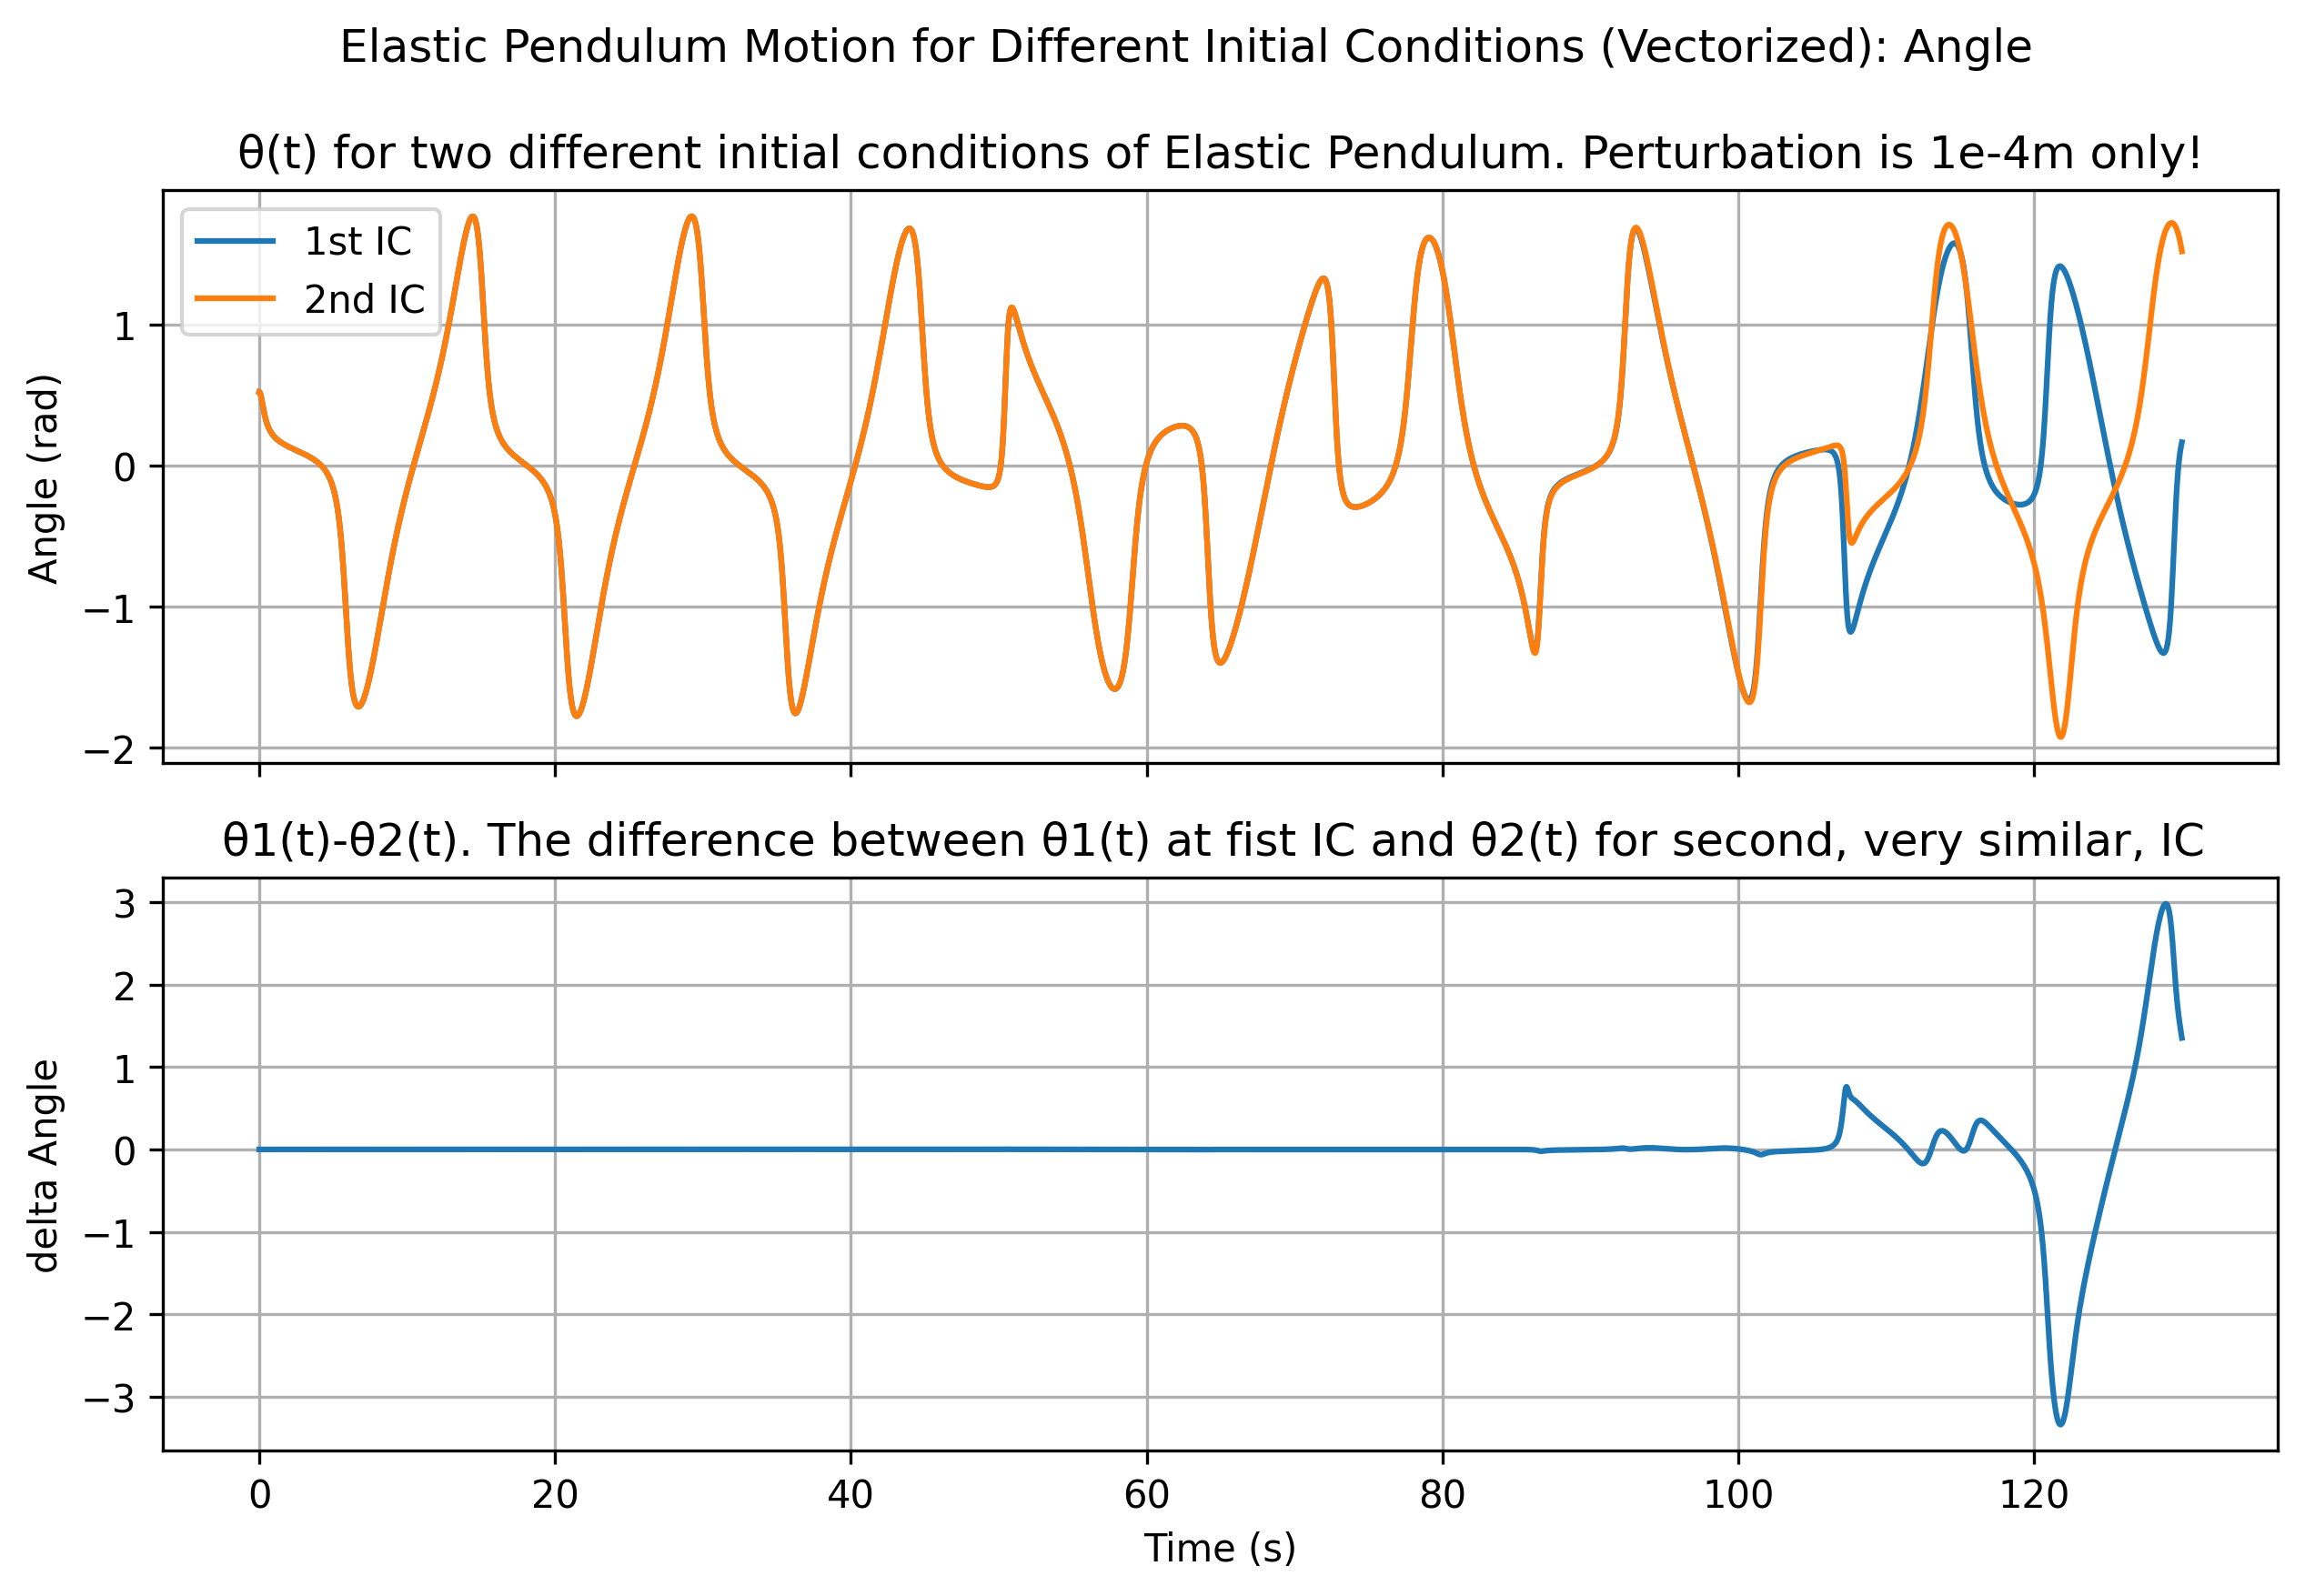
\includegraphics[width=0.8\textwidth]{elastic_pendulum_theta.png}
				\caption{Angle and difference over time}
		\end{figure}
	\end{enumerate}
	
	\section*{II. Energy Conservation Plot}
	
	\begin{figure}[h!]
		\centering
		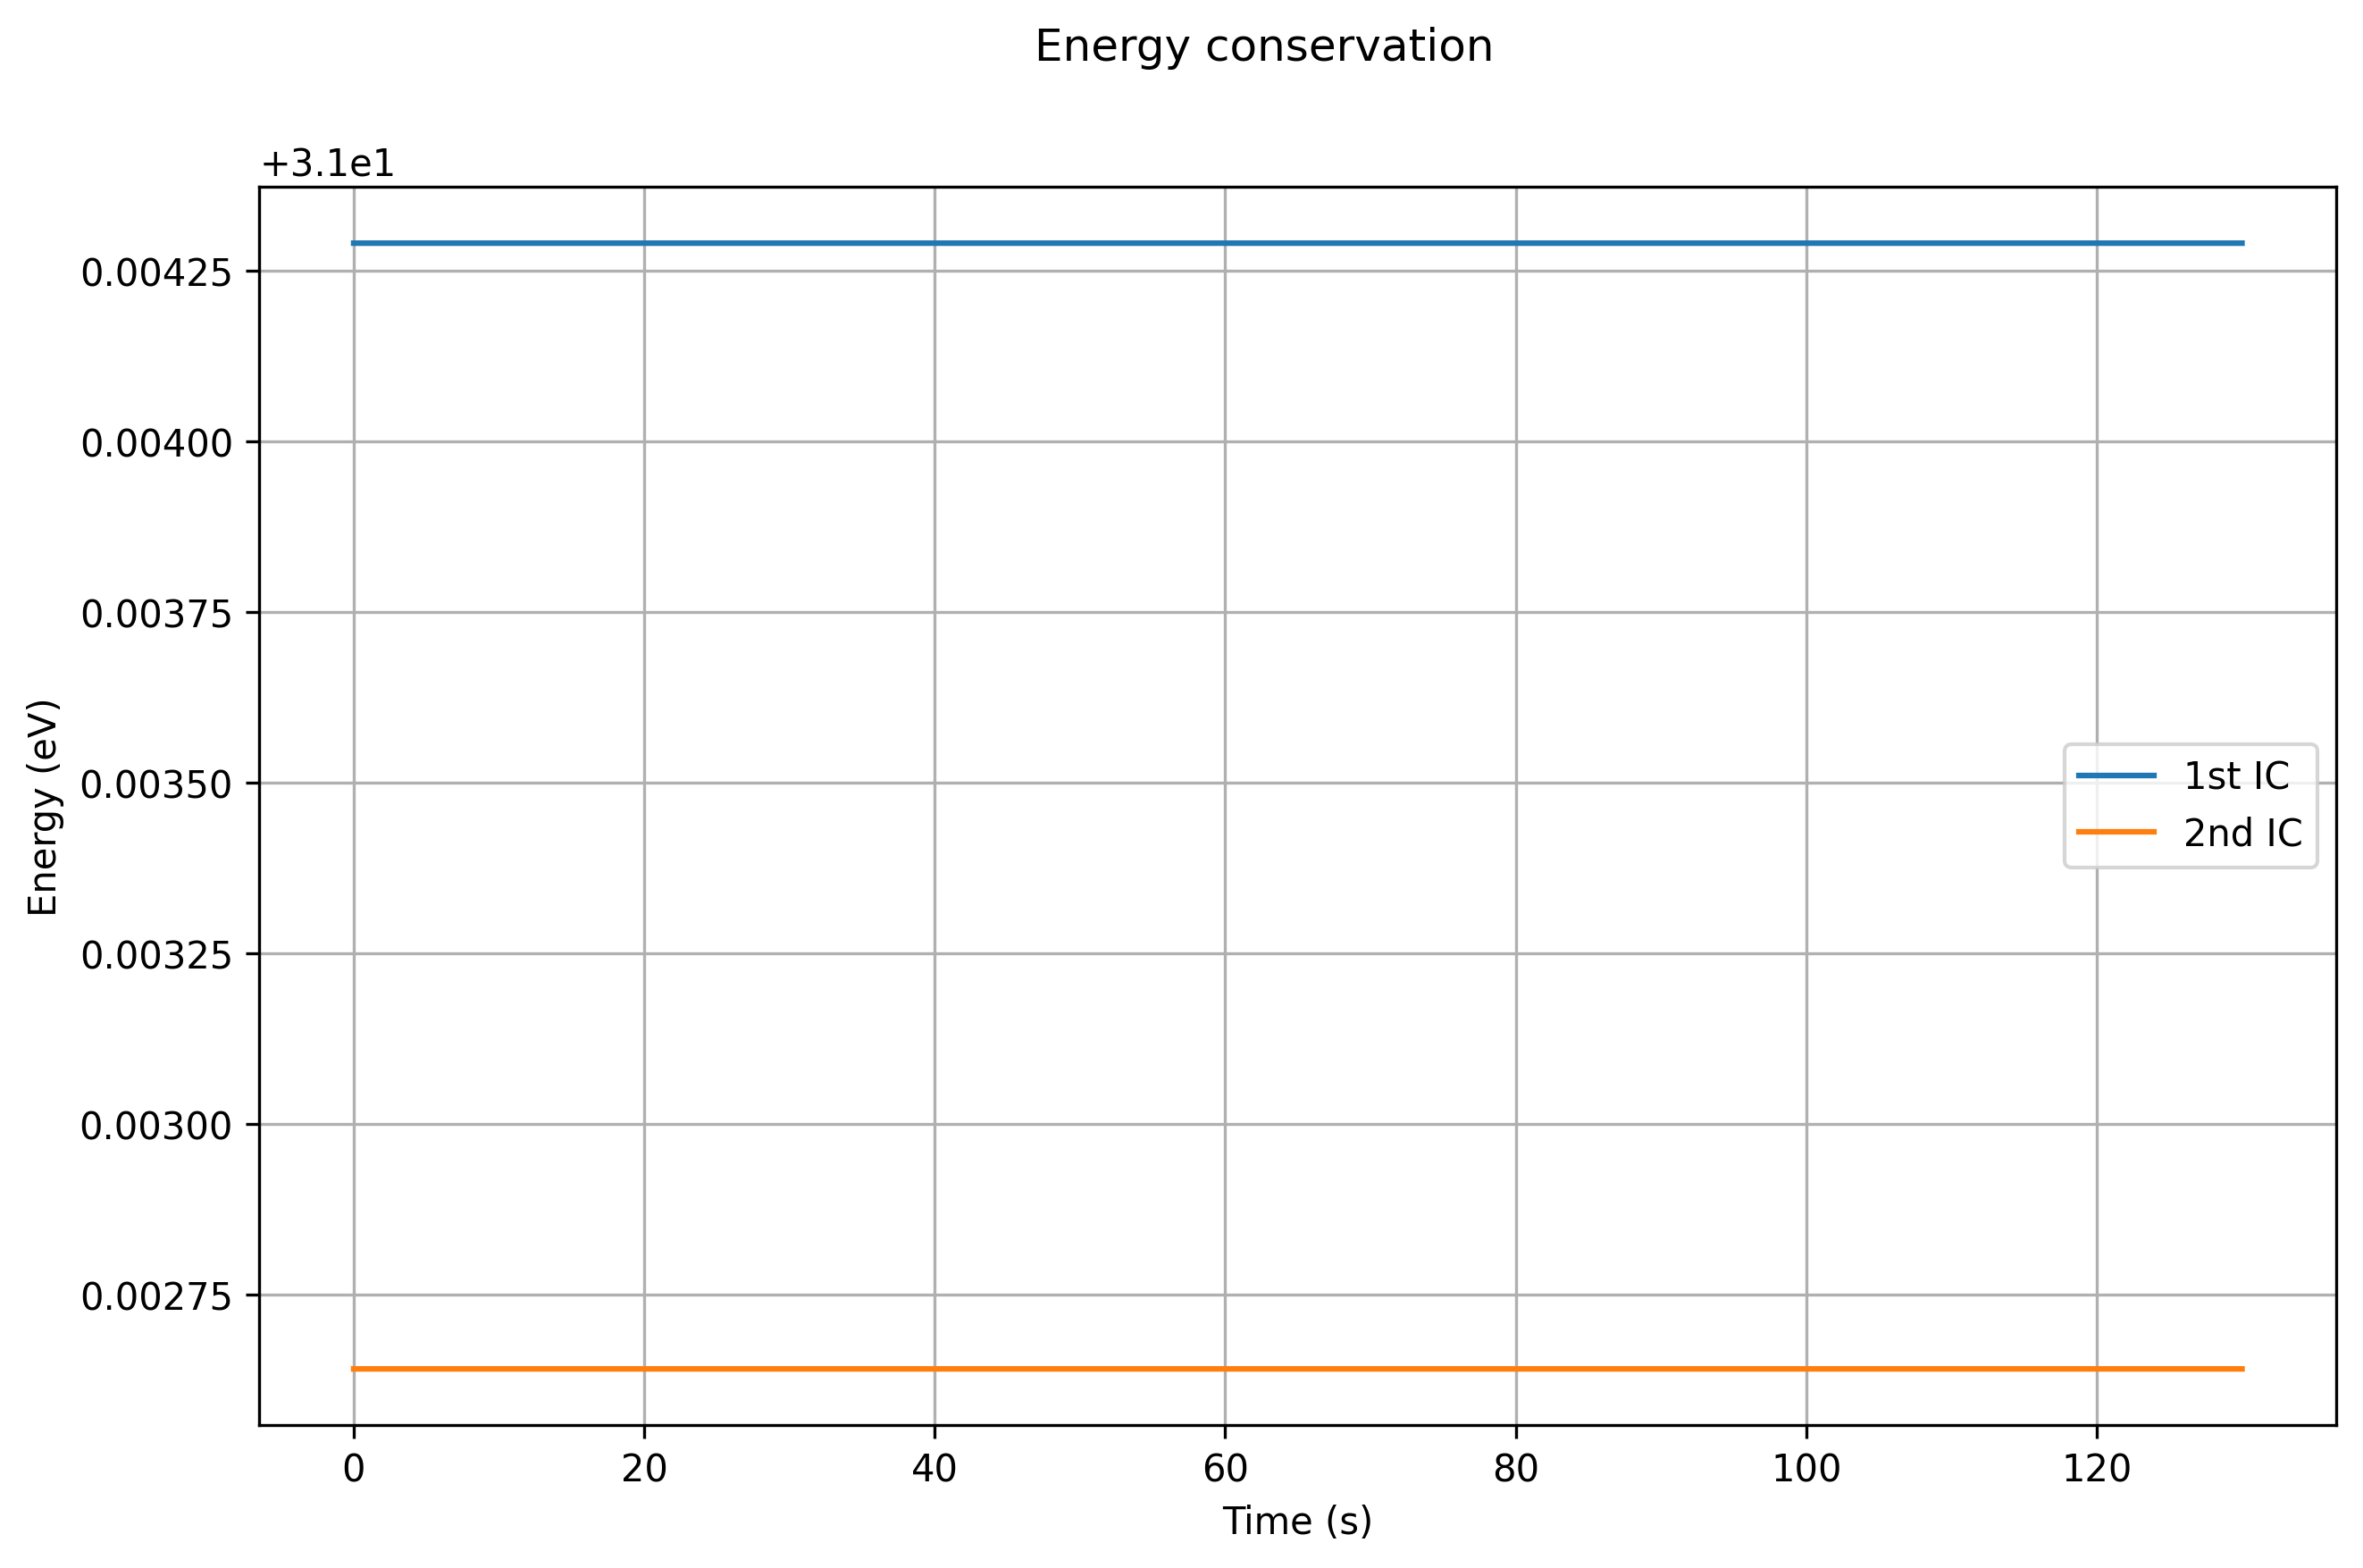
\includegraphics[width=0.9\textwidth]{energy.png}
		\caption{Energy Conservation}
	\end{figure}
	
	Energy conservation is maintained numerically due to the conservative nature of the pendulum system. Total mechanical energy (kinetic plus potential energy) remains constant, indicating correct numerical integration.
	
	\section*{III. Lyapunov Exponent Analysis}
	
	\begin{enumerate}
		\item The logarithmic-scale chart of $||\delta_Y||$ (norm of differences) is presented below:
		
		\begin{figure}[h!]
			\centering
			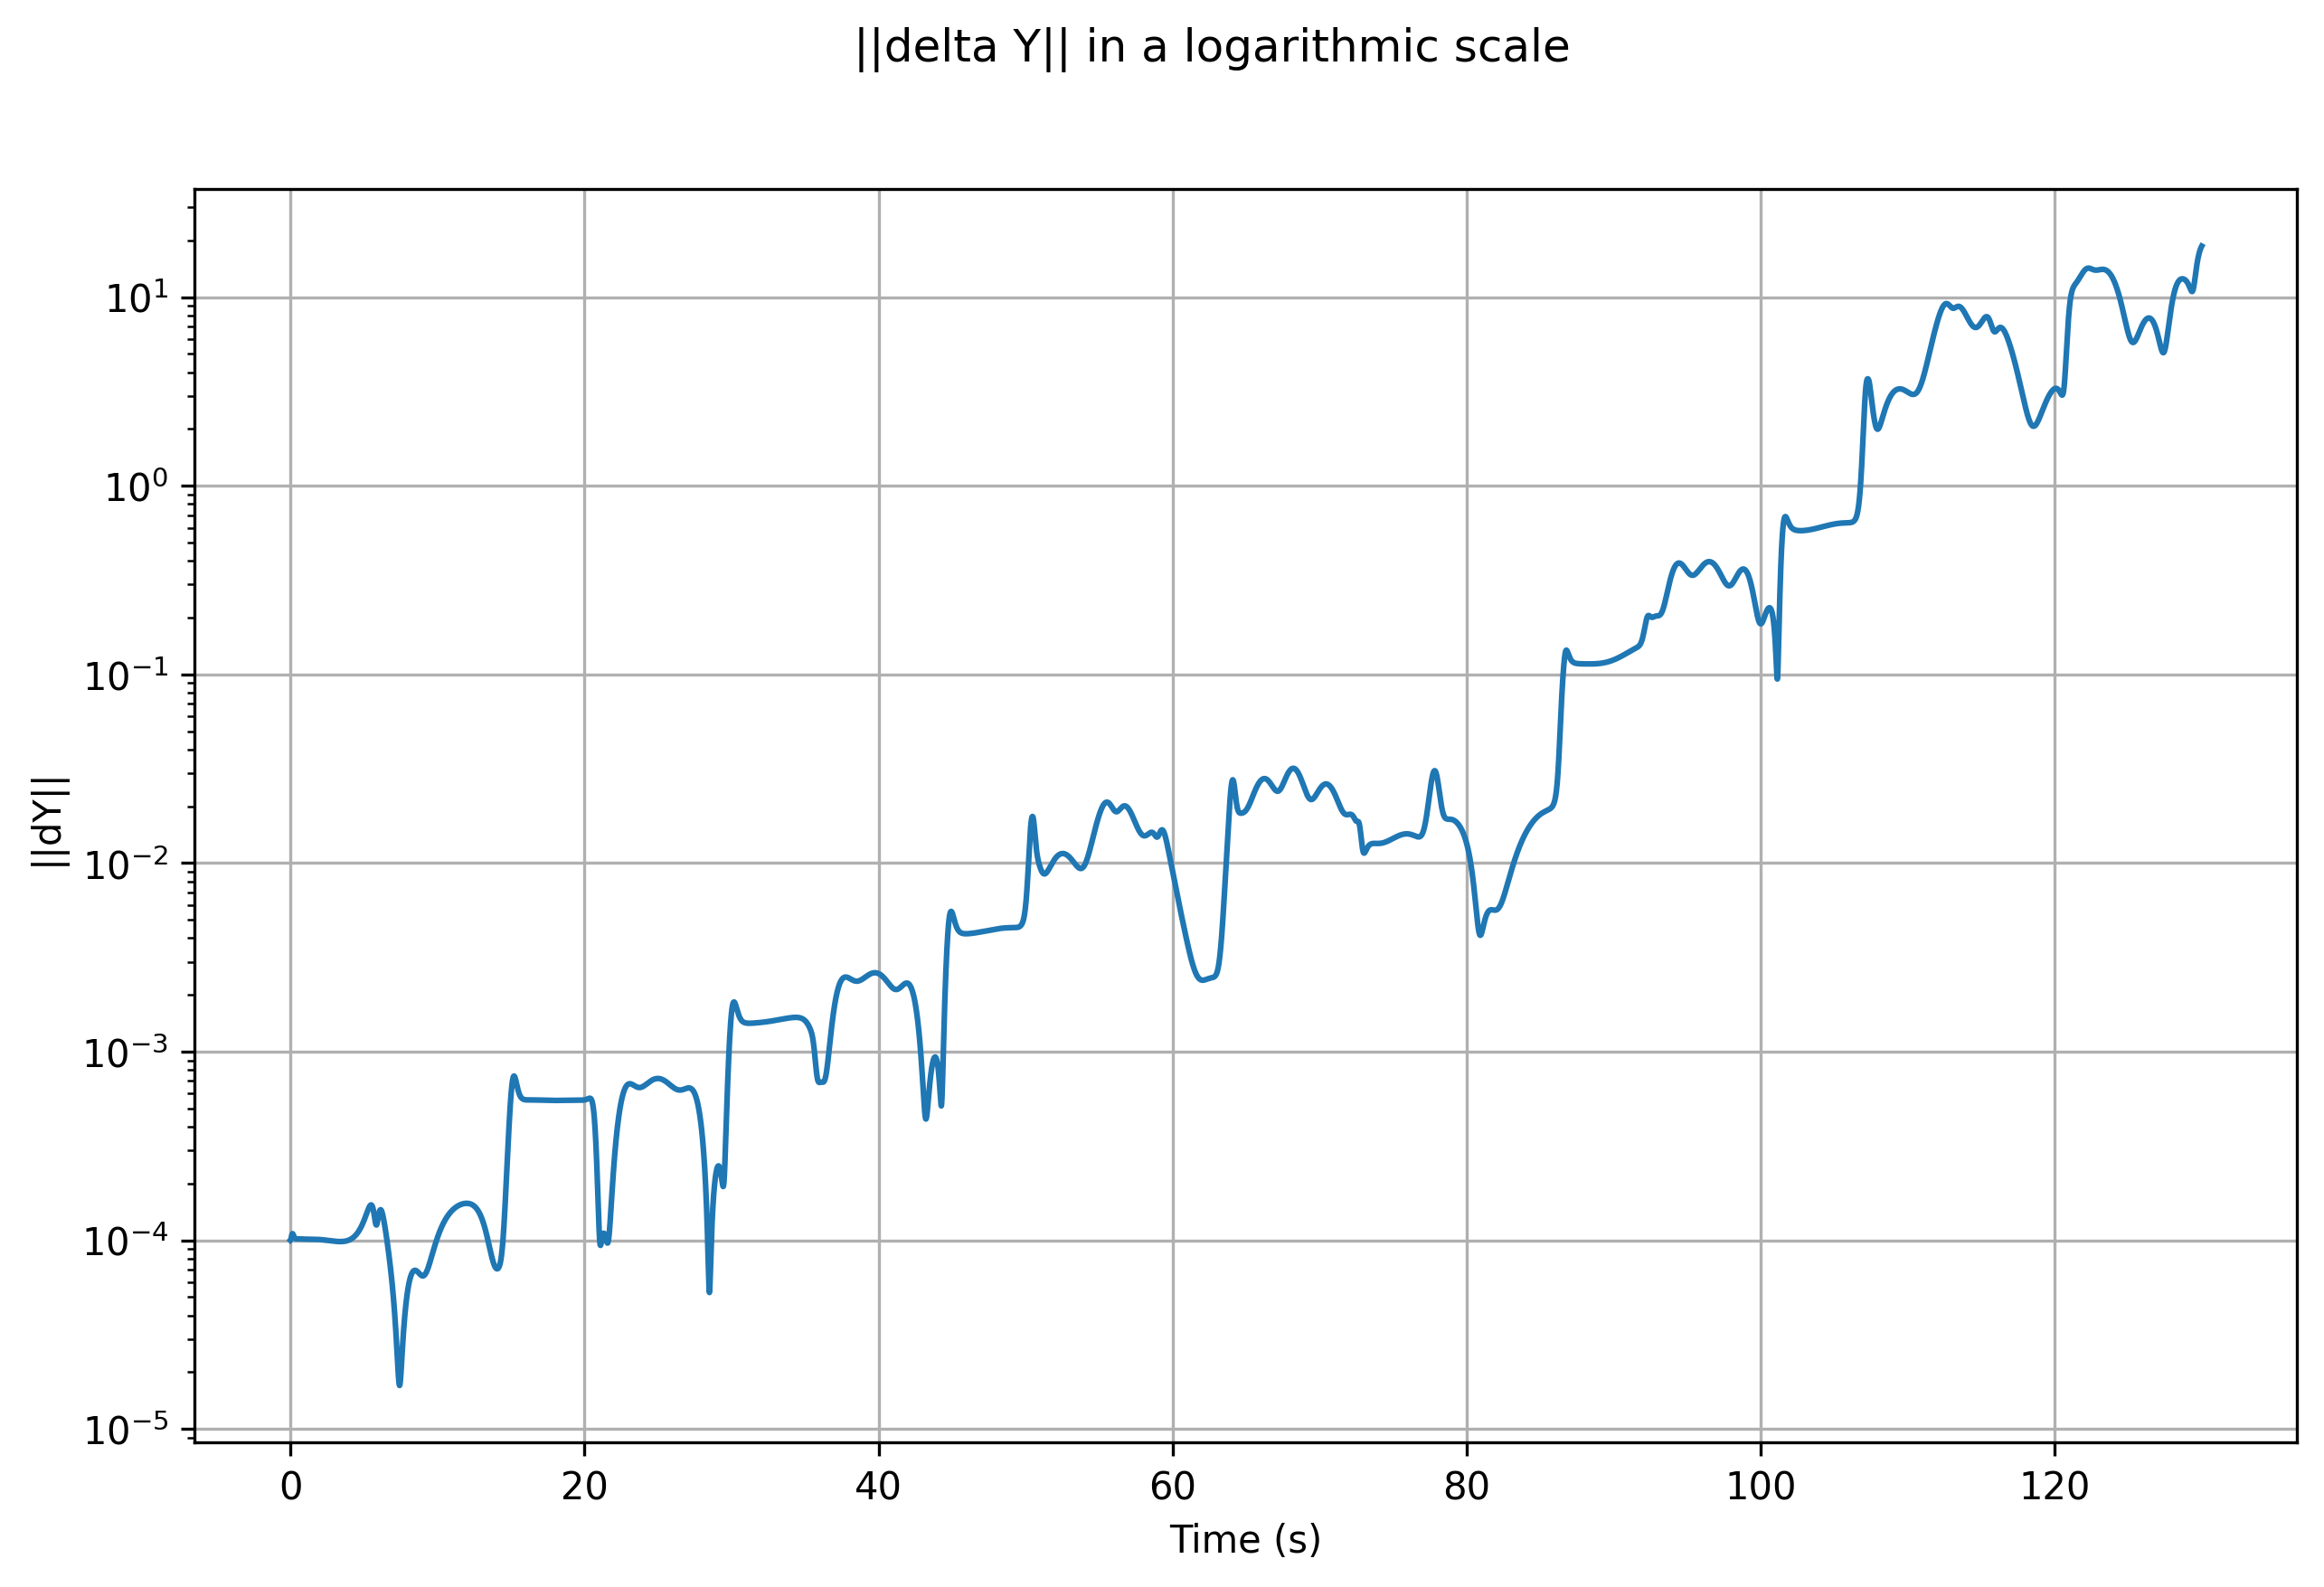
\includegraphics[width=0.9\textwidth]{norma_of_delta_Y.png}
			\caption{Logarithmic Scale of $||\delta_Y||$}
		\end{figure}
		
		\item The straight-line appearance on the logarithmic scale chart indicates exponential divergence, allowing the use of the Lyapunov exponent formula:
		\[
		\lambda = \frac{1}{t_{\text{max}}}\log\frac{||\delta_Y(t_{\text{max}})||}{||\delta_Y(0)||}
		\]
		
		\item The Python implementation in \texttt{elastic\_pendulum.py} integrates the variational equations alongside the original trajectory to calculate divergence and estimate the largest Lyapunov exponent. Initial perturbation and trajectory divergence are numerically tracked, followed by fitting to an exponential model to extract $\lambda$.
		
		\item The provided Python code used for calculating the Lyapunov exponent is attached in \texttt{elastic\_pendulum.py}.
	\end{enumerate}
	
	\section*{IV. Poincaré Section Visualization}
	
	\begin{enumerate}
		\item The Poincaré section was computed using \texttt{poincare\_section.py}, sampling trajectory points where $\theta = 0$ with $\dot{\theta} > 0$.
			\begin{lstlisting}
			See attached script poincare_section.py.
			I do know how to quote the code in LaTex.
			\end{lstlisting}
			
		
		\item The resulting Poincaré section chart is shown below:
		
		\begin{figure}[h!]
			\centering
			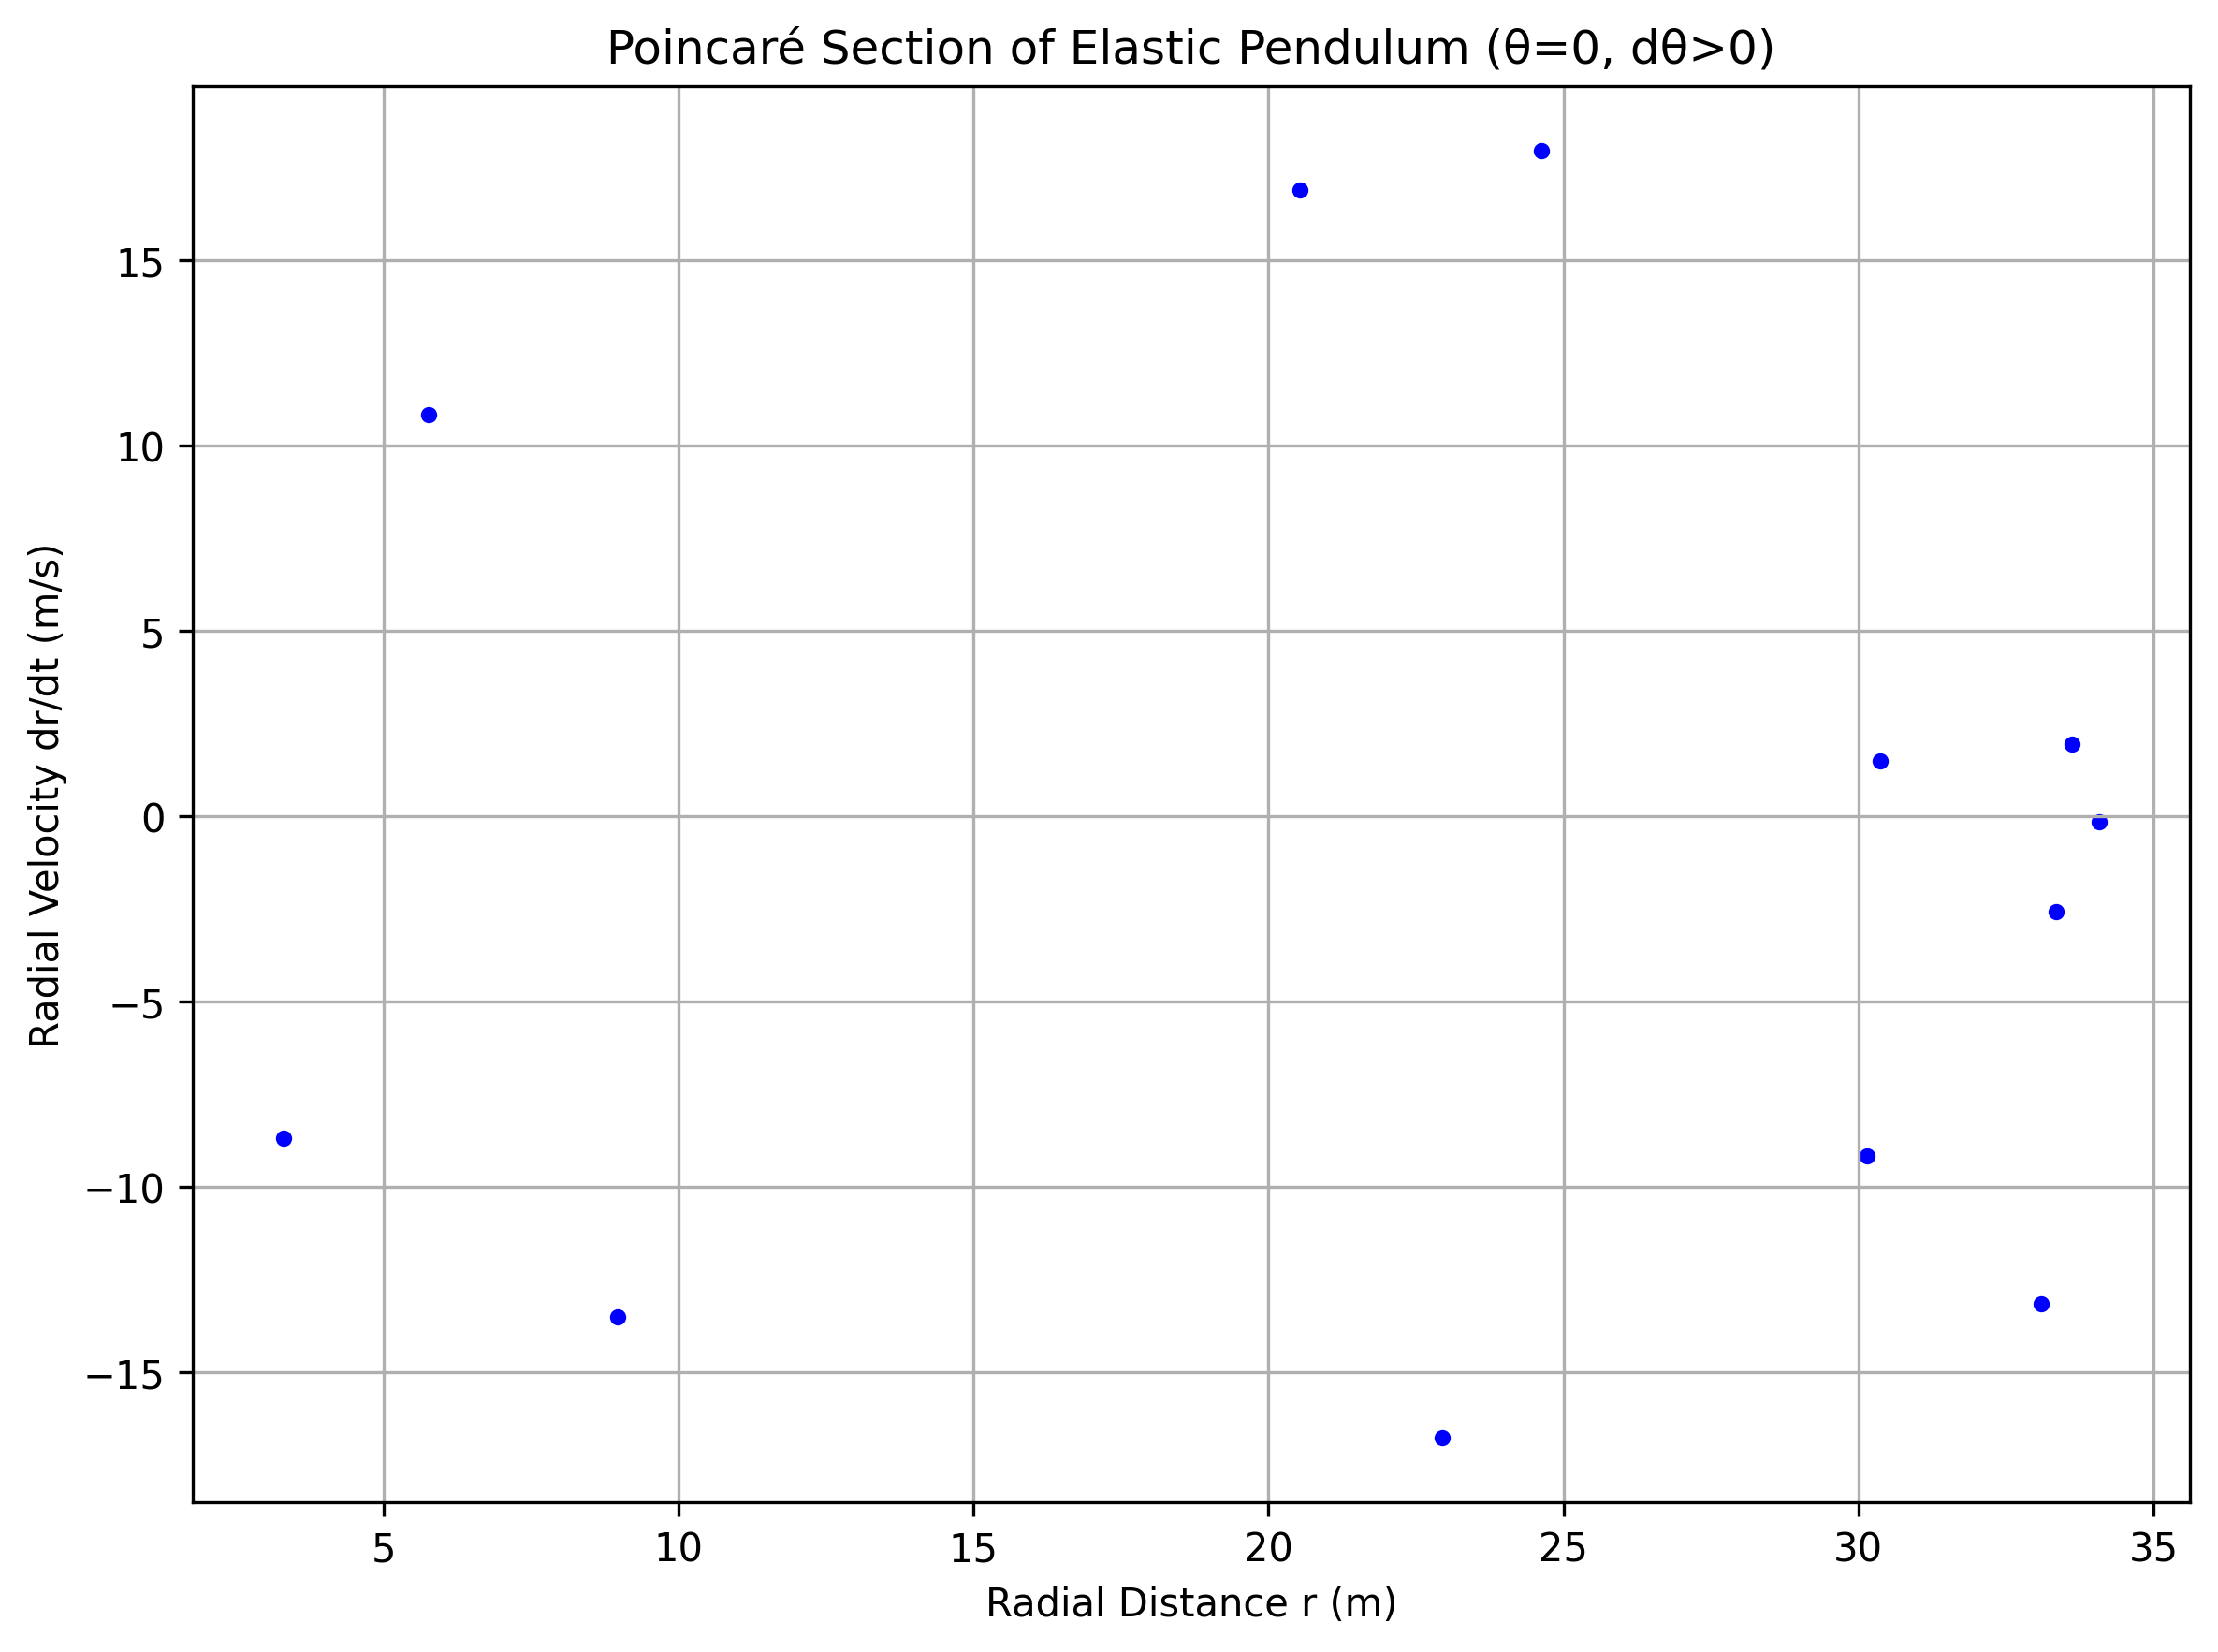
\includegraphics[width=0.8\textwidth]{poincare_section.png}
			\caption{Poincaré Section}
		\end{figure}
		
		\item The chart reveals the intricate phase space structure, displaying patterns indicative of both regular and chaotic regions. The conditions defining this section ($\theta = 0$, $\dot{\theta} > 0$) facilitate clear observation of the system's dynamics.
	\end{enumerate}
	\pagebreak
	
	\section*{V. Discussion on Chaotic Behavior}
	
	\begin{enumerate}
		\item The chaotic dynamics of the elastic pendulum are evident from the first chart on \texttt{Figure 6}, highlighting irregular oscillations in $\theta(t)$.
			\begin{figure}[h!]
				\centering
				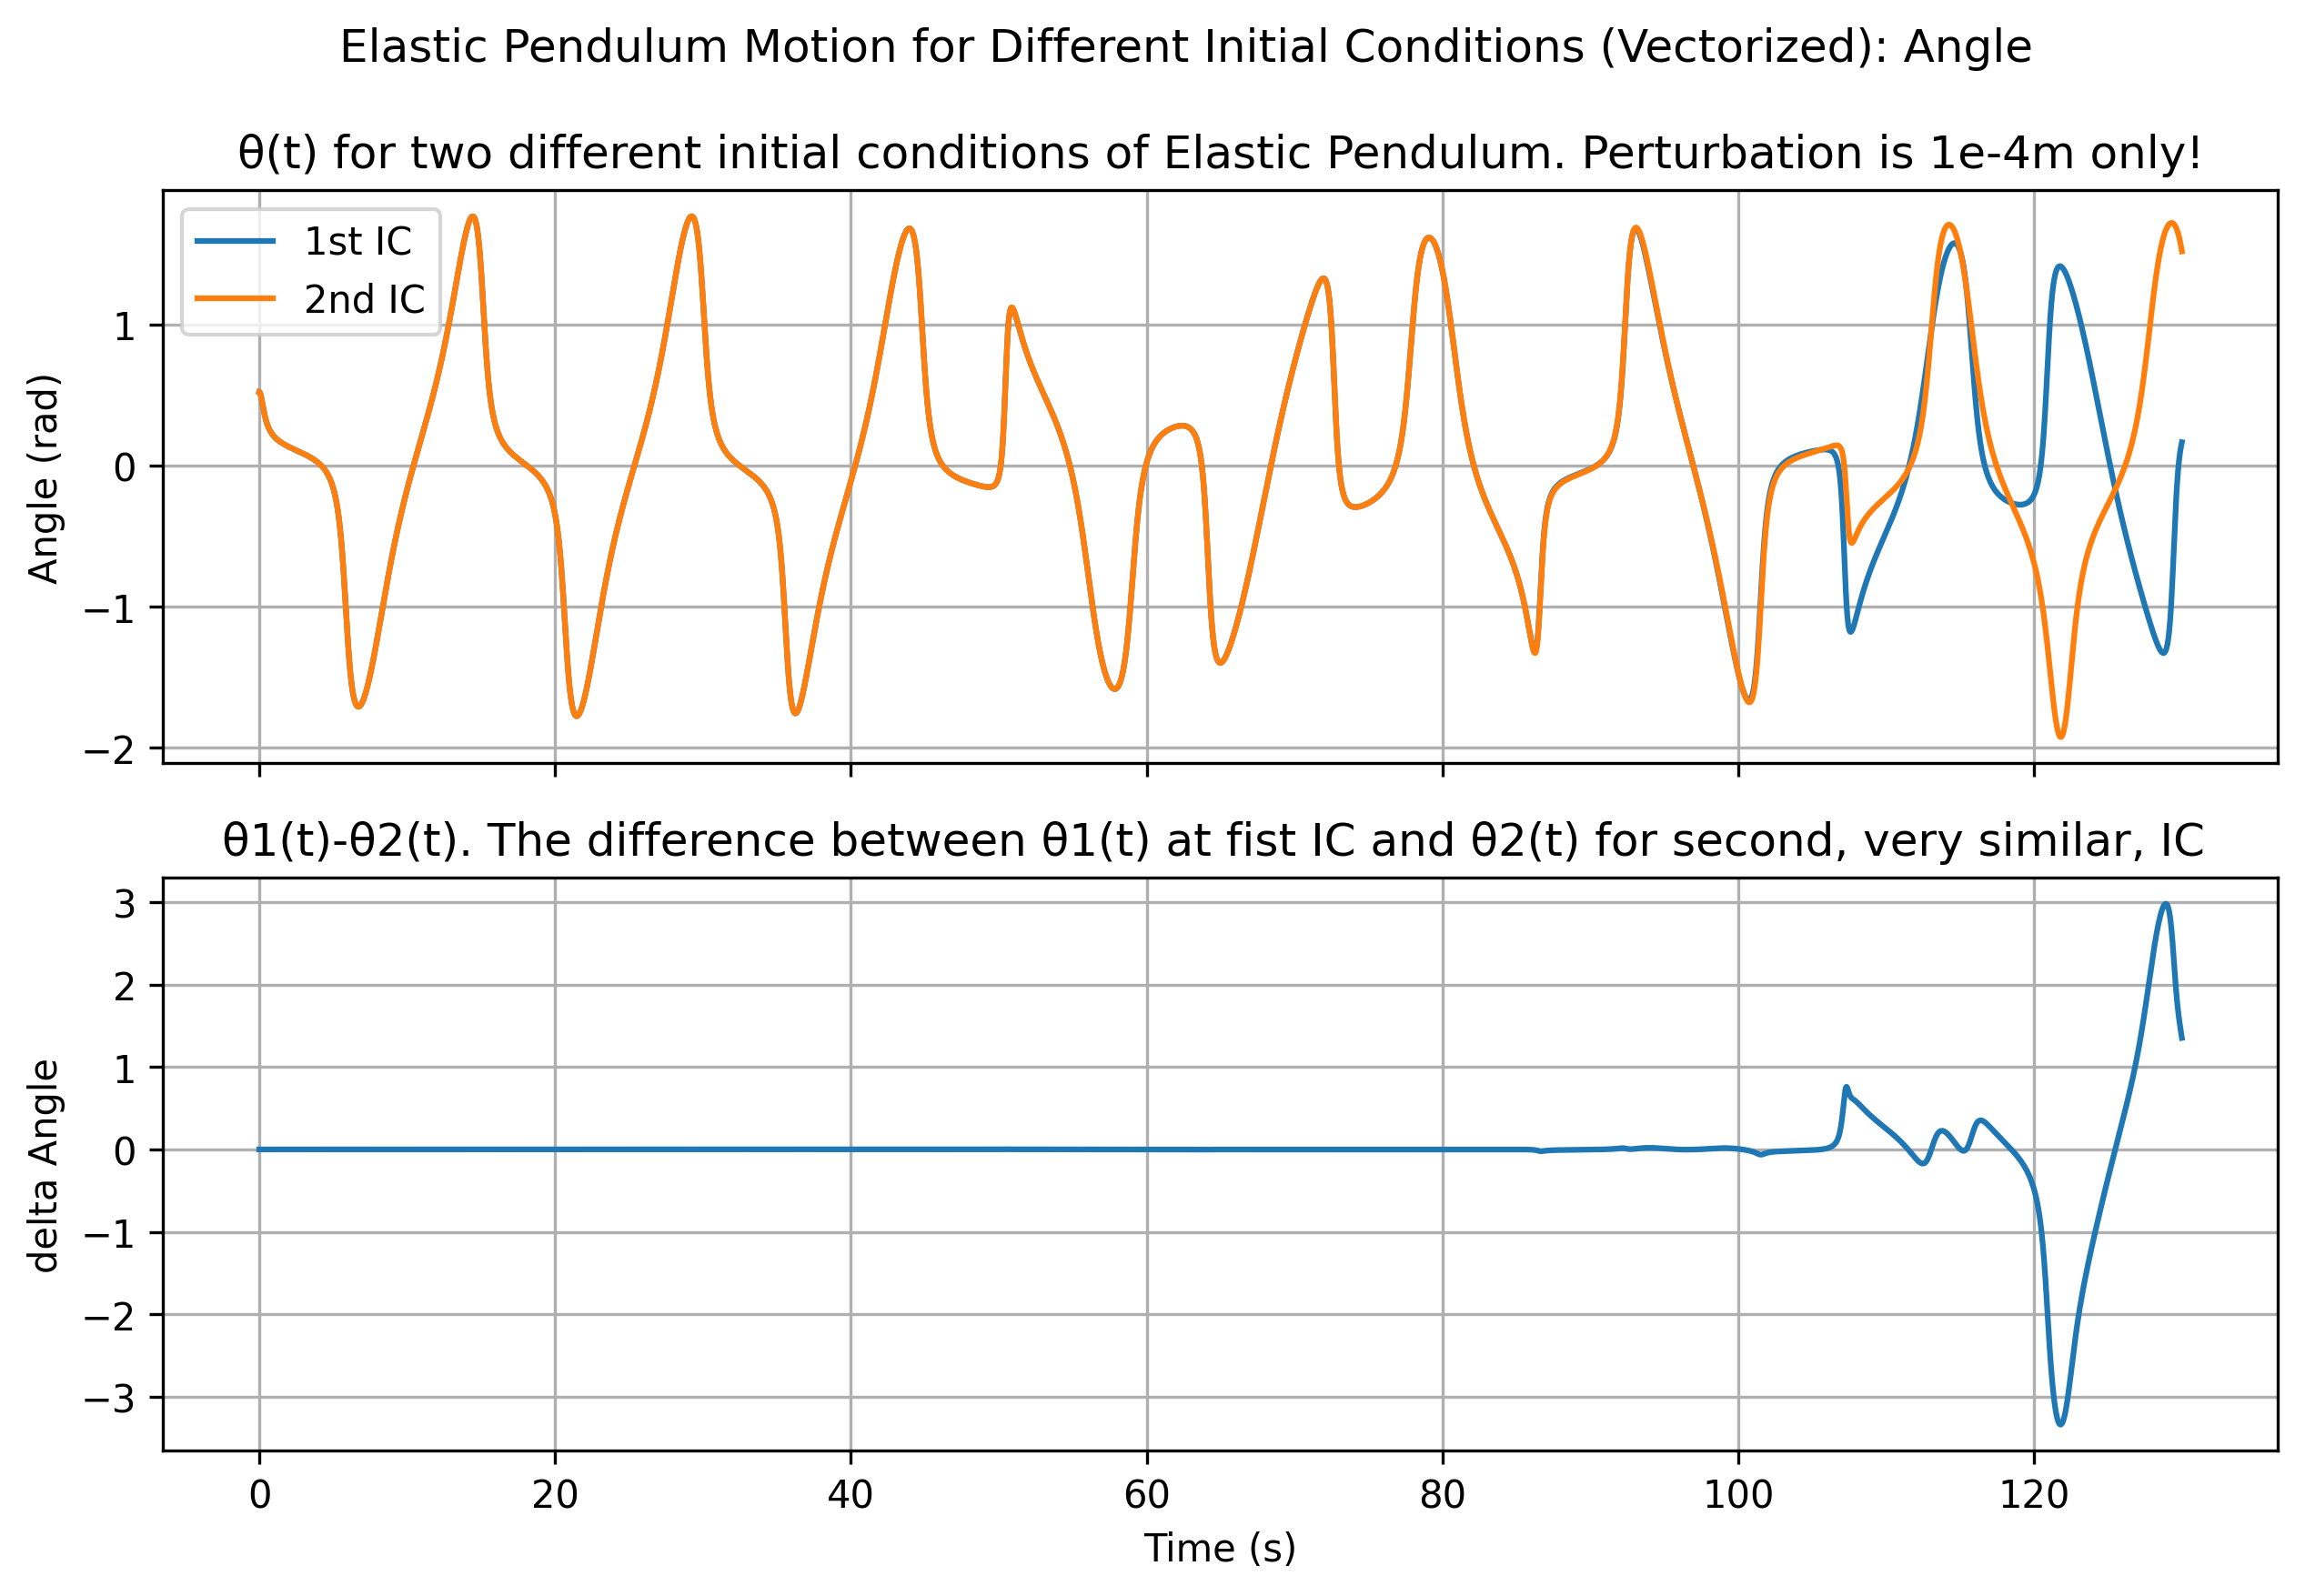
\includegraphics[width=0.9\textwidth]{elastic_pendulum_theta.png}
				\caption{chaotic dynamics of the elastic pendulum}
			\end{figure}
		
		\item Chaotic behavior arises due to the nonlinear interactions between radial and angular modes, creating a sensitive dependence on initial conditions. Small perturbations are rapidly amplified through the nonlinear coupling, generating complex and unpredictable trajectories.
	\end{enumerate}
	
\end{document}

